\section{Fame data computational methods}
\label{app:data-cleaning}

The following section provides detailed guidance for the data manipulation undertaken in this analysis.
I emphasise reproducibility due to the discussion on \fullref{s:intro}:
this analysis offers a substantive baseline with advanced data science techniques and econometric methods,
on top of which I leave it for future analysis to carry out the more sophisticated extensions of section \ref{s:extensions}.
All scripts are publicly available
online\footnote{https://github.com/aloysiuslip/ucl-diss-ECON0079},
written in Python and Jupyter notebooks.

\subsection{Data cleaning procedure}
\label{app-ss:financial-data}

\itx{DuckDB} operates locally, meaning minimal lag from issuance to execution time
provided the operating machine is sufficiently high-compute,
and stores data in column vectors, which is a significant advantage
to manipulating whole variables.
Any SQL commands issued from the Python are compiled down to C,
making execution for column transformation operations extremely fast,
even for joining tables of several 100s of millions of rows\footnote{Explanatory
numbers given in this section are rounded to 3 significant figures for ease},
as is calculated in this analysis for target-peer spatial distances.
I wrote database interaction commands using \itx{Ibis},
an Apache-2.0 licensed Object-Relational Mapping (ORM) framework
which allows SQL commands to be written natively in Python\footnote{\cite{TheIbisProjectAuthors2026}},
minimising the likelihood of errors when issuing queries loops or changing variable names.
This architecture choice is extremely well-suited for mass data econometric analysis
and critical to solving the compute limitations of iterative large-$n$ dataset manipulations
required to calculate the valid instruments identified in section \ref{ss:static-identification}.
\par
Raw data are distributed across a series of Excel files on balance sheet indicators,
including time-invariant characteristics for each firm, bucketed into $a1\_ID$ and $a5\_misc$ files,
and annual data published on a calendar-year basis,
bucketed into \itx{a2\_key\_finance}, \itx{a3\_assets}, and \itx{a4\_profits} tables.
\par
I traversed the file structure to build a dictionary to the filepaths organised in their subfolders,
which are named by the 2-digit industry SIC division,
and batch-imported data belonging to the firms in that industry.
Some industries have prodigious registered firms,
such as SIC division 47 (Retail Trade, 1090 files)
and 82 (Office administrative, office support and other business support activities,
1065 files)\footnote{\cite{ons2026:sic}}.
I imposed a batch limit of 200 for stable memory handling, splitting up these large industries,
and used Python's asynchronous \itx{concurrent.futures} package
to execute the ingestion of each batch, exploiting multithreaded processing.
In total, 12,800 files were processed across the 88 available SIC divisions.
Time-invariant firm characteristics were saved to a table named \itx{fixed},
annual firm data to a table named \itx{yearly} within \itx{DuckDB}.
\par
All firm data are tagged with a \itx{registered\_number} property corresponding to a Companies House ID.
I deduplicated 896,000 \itx{fixed} firm entries using a \itx{registered\_number} match,
of which the vast majority were exact duplicate entries
and the remainder had some mismatch of 1 or more firm characteristics,
such as the listed company name, global operating owner,
and in rare cases, location.
Duplicate entries are an undesirable feature of the Fame dataset,
worsened by Fame's construction from snapshots of reported firm data
across timepoints, where resolution of conflicting \itx{fixed} data may be imperfect.
Fame also contains data impute errors, meaning variations in names referring to the same entity.
When duplicates occurred, I effectively randomly chose an entry to keep.
A more robust analysis could devise further data science methods,
such a deployment of an acceptable Levenshtein distance to resolve differing name entries,
or separately treating firms with multiple listed addresses.
Further data cleaning procedures are discussed in \cite{Irastorza-Fadrique2026}, notably these include
avoiding double-counting of firms through both their parent company and subsidiaries,
truncation of data to at earliest 2010 due to changes in reporting standards,
and reclassification of firm SIC codes using NLP on firm business activity descriptions.
\begin{figure}[b!]
    \caption{Panel observation availability by year}
    \label{fig:data-obvs-per-year}
    \centering
    \graphicspath{{../../descriptives/output/}}
    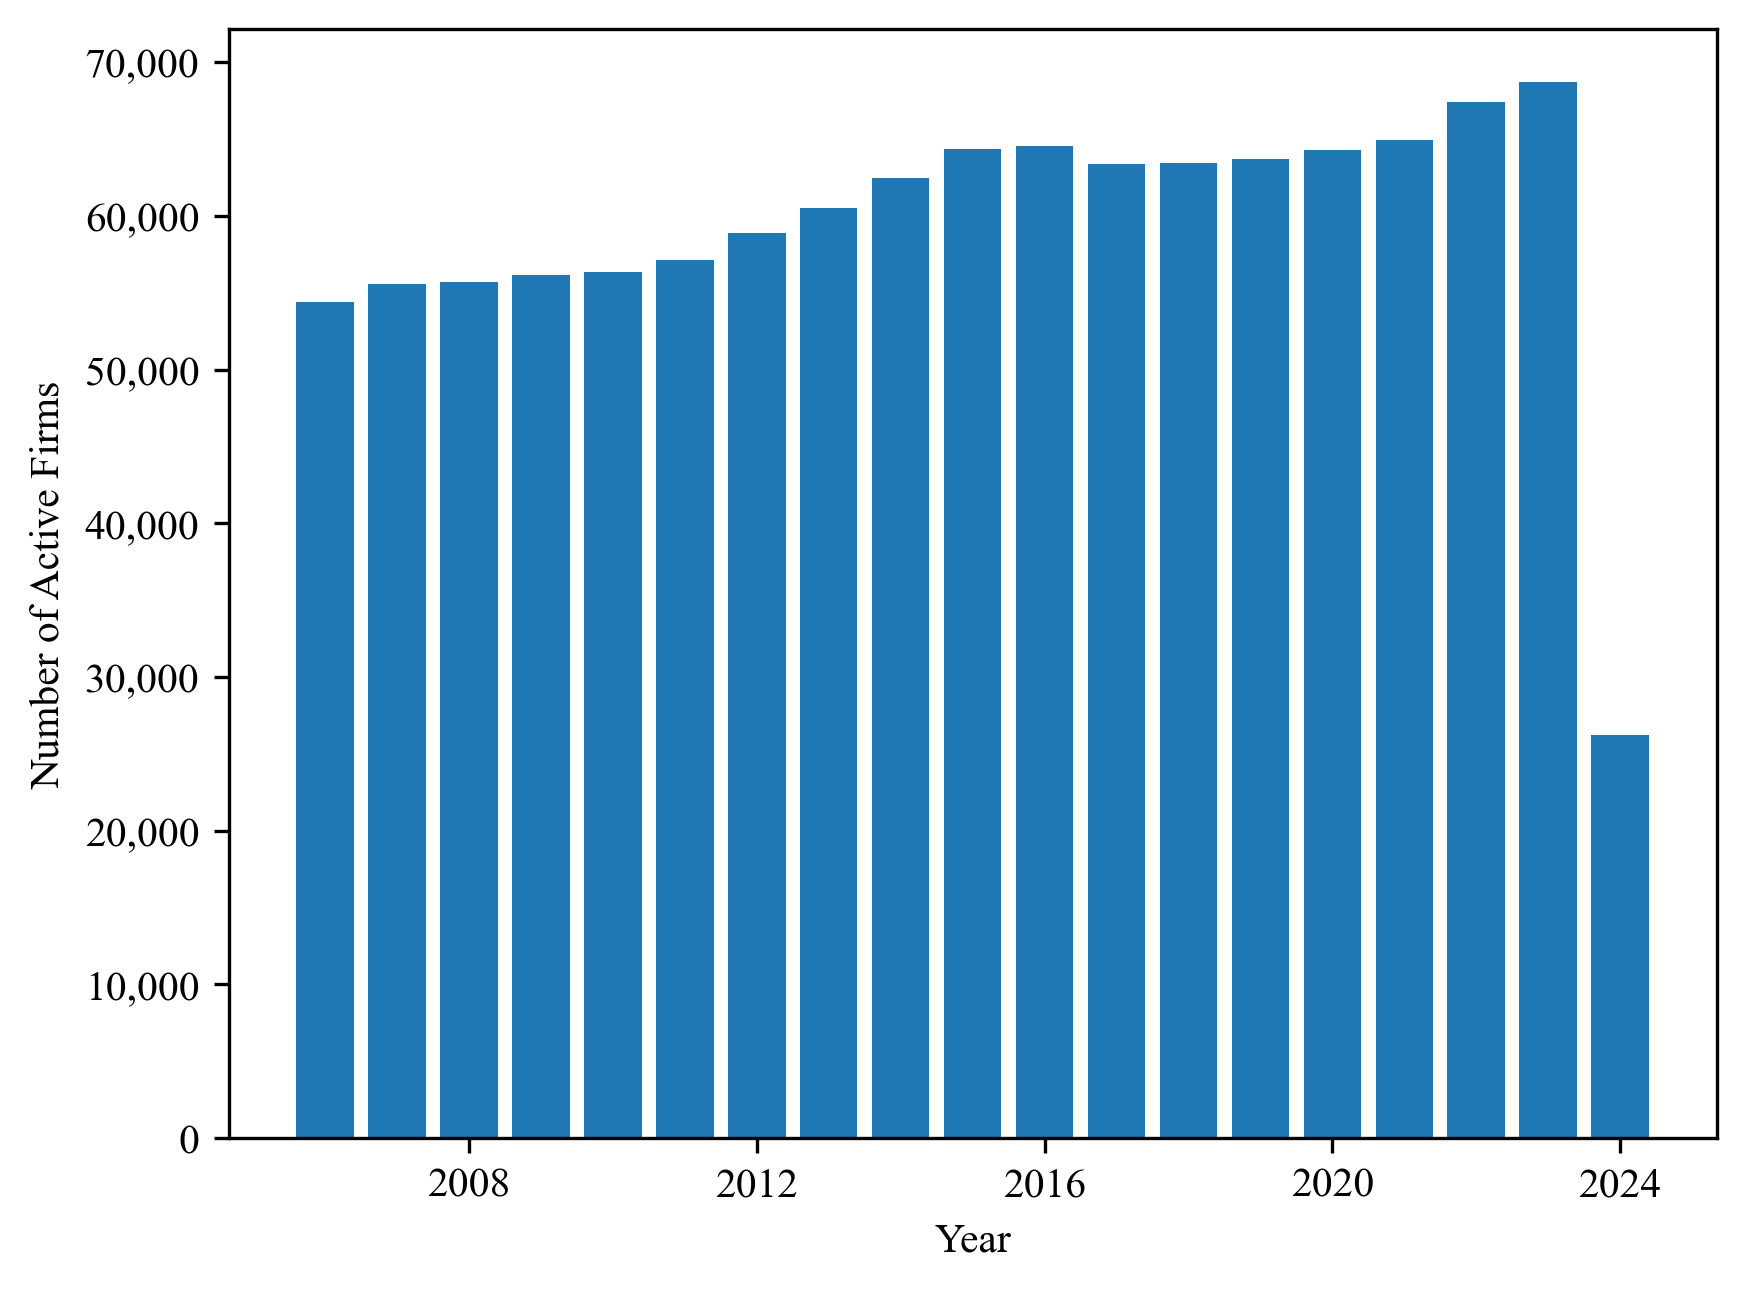
\includegraphics[width=\textwidth]{fig_panel_obvs_by_year.png}
    \caption{Distribution of years of data available per firm}
    \label{fig:data-years-per-firm}
    \centering
    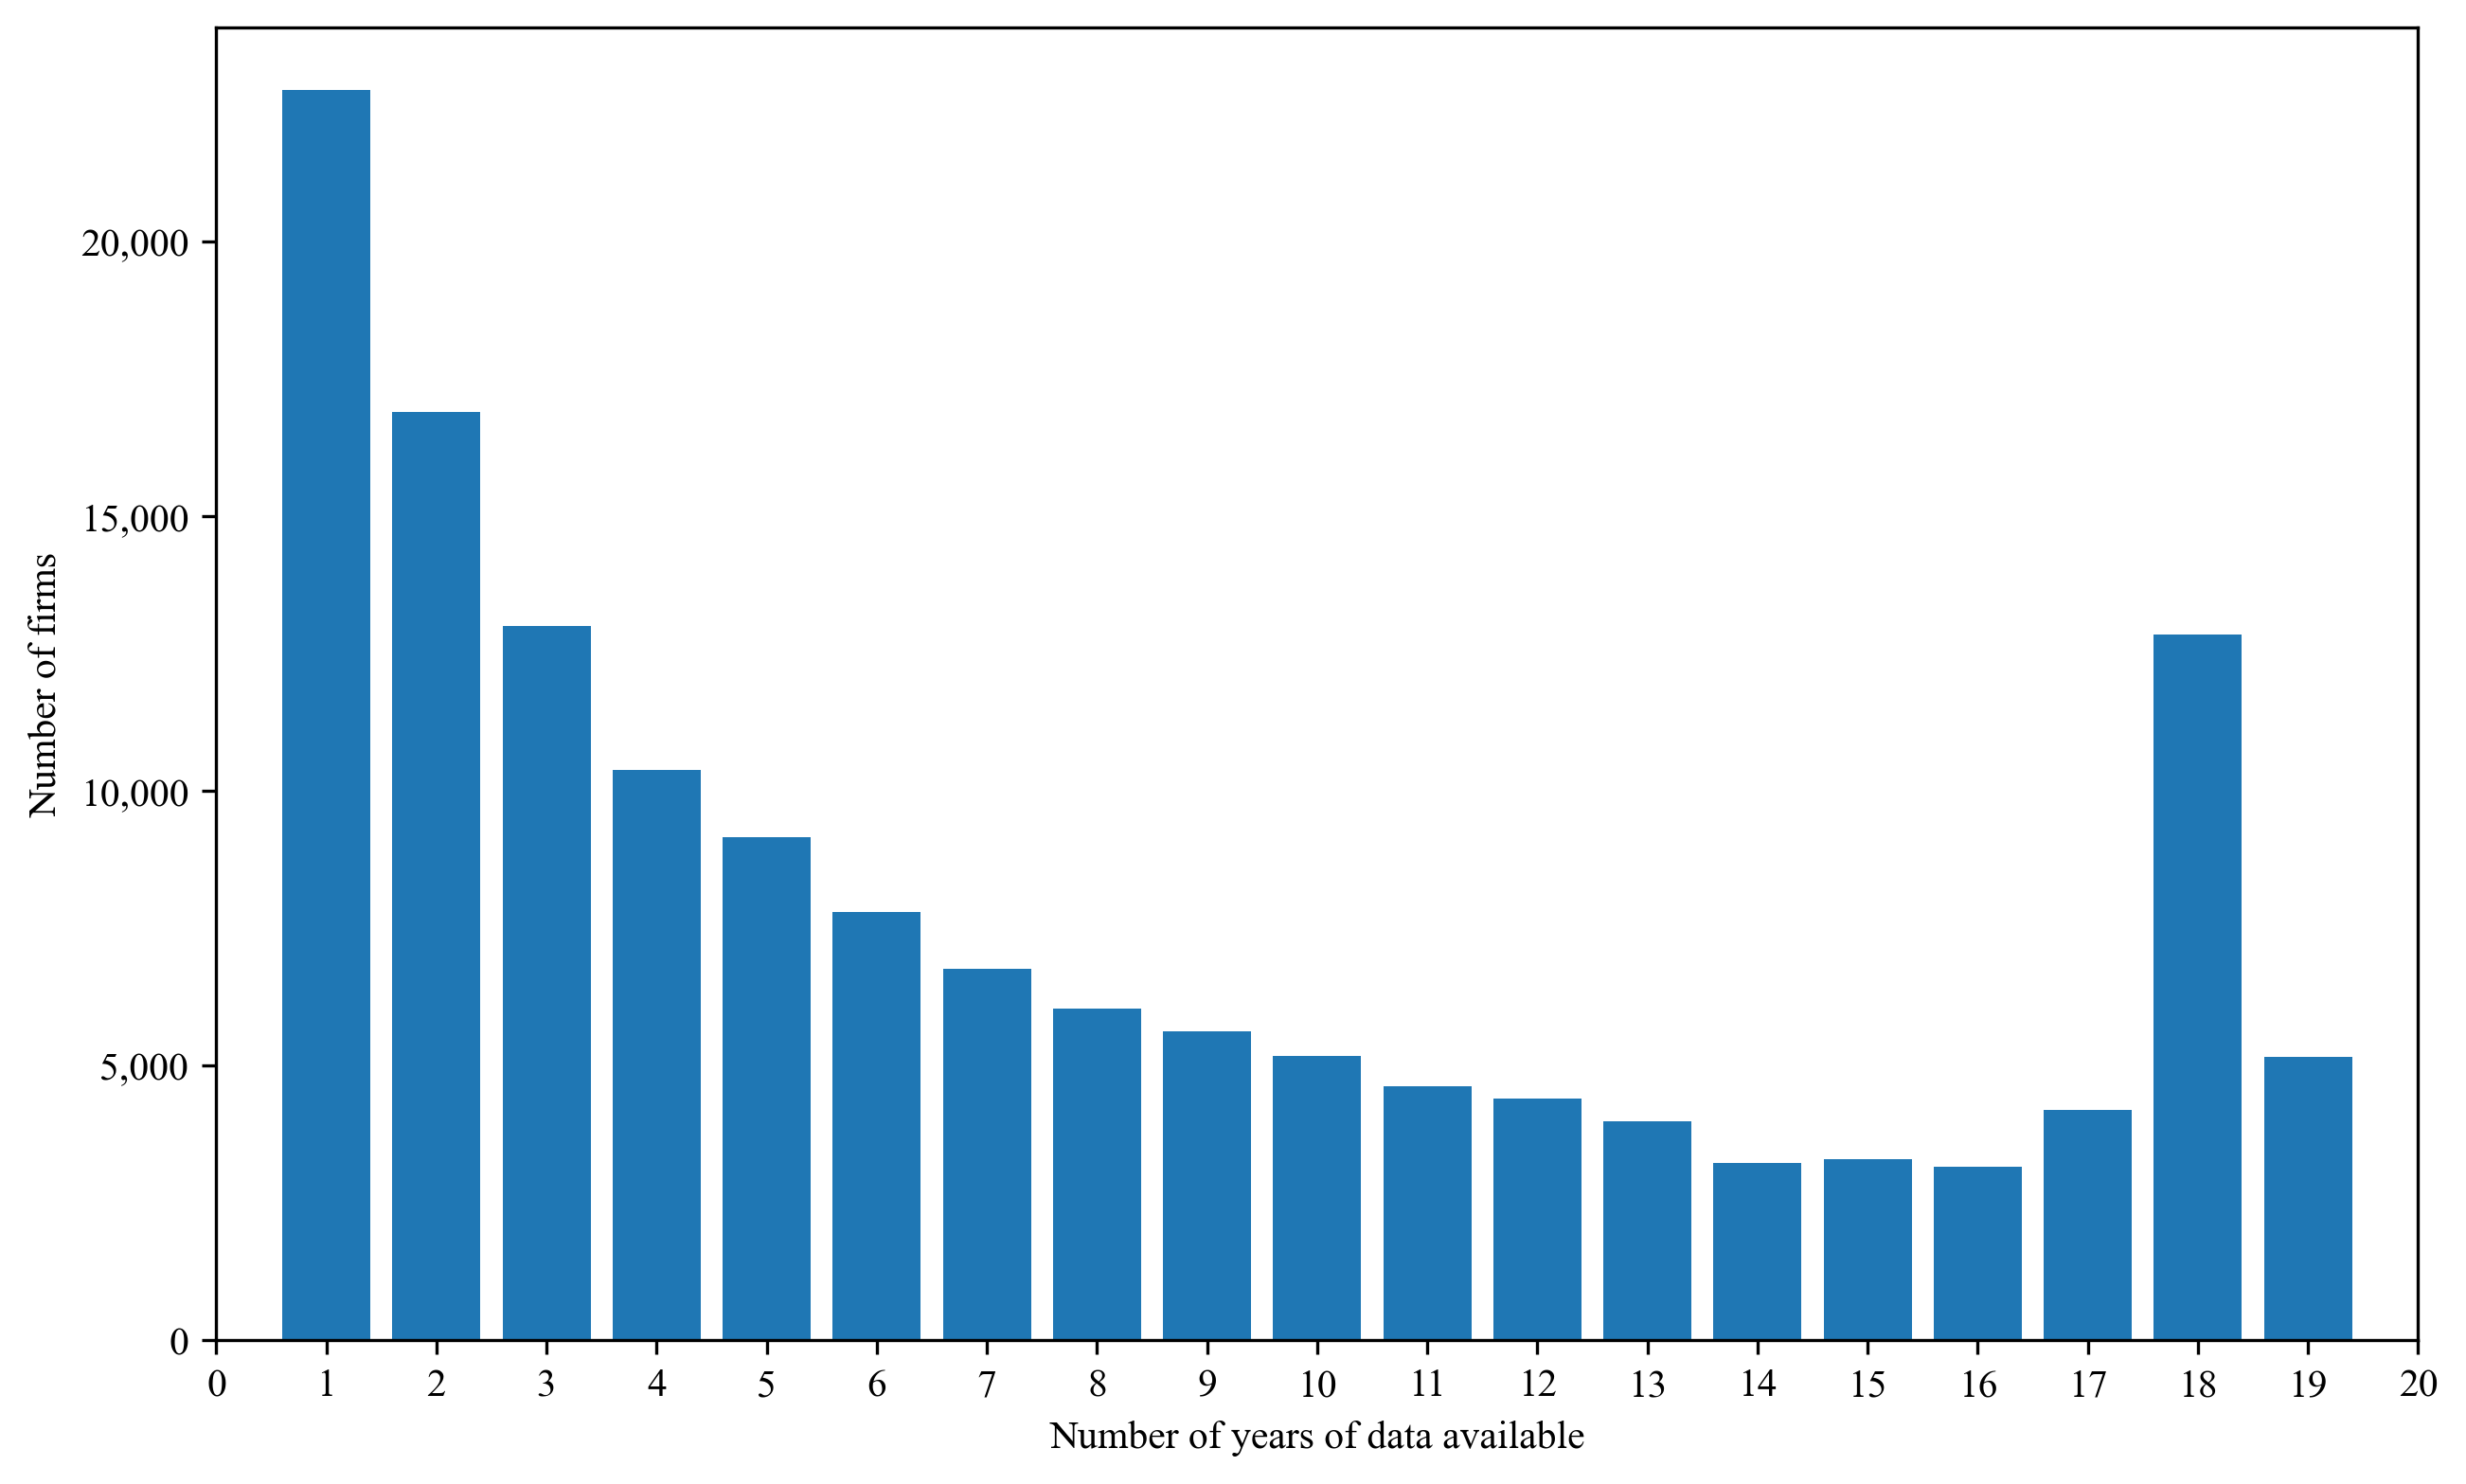
\includegraphics[width=\textwidth]{fig_panel_years_avail.png}
    \begin{tablenotes}
        Fame panel sample downloaded from calendar years 2006 to 2024 inclusive.
        Firms with zero years of data available filtered out.
        Sample downloaded February 2025, resulting in incomplete reporting for 2024.
    \end{tablenotes}
\end{figure}

As the main analysis here only uses location data as the \itx{fixed} characteristic of analysis,
due to its time constraints, and due to the low number of duplicates
and other cleaning errors listed above relative to the size of the dataset,
I treat those errors as random effects and deem the impact of the random selection strategy minimal.
I similarly removed duplicate firm-year entries in the \itx{yearly} data,
and merged the two tables based on ensuring every \itx{fixed} firm identity
had a corresponding \itx{yearly} set of rows, and vice versa.
For efficiency, I adopted a `max-merge' column strategy,
which is effective for resolving entries which are zero and non-zero in conflicting duplicates.
This however means that any two observations with conflicting non-zero values keep the large value.
If it is random errors causing Fame to have these conflicting, duplicate values,
this strategy has the potential to bias all financial data entries upwards,
however this bias is unlikely to be correlated with any of this investigation's variables of interest.
I further removed a small minority (<200) firm entries not based in the UK,
which can be identified through their \itx{registered\_number} format.
In total, deduplication reduced the number of firms from 9,280,000 to 8,220,000,
and the number of panel observations from 44,900,000 to 42,900,000.

\par
I restrict the sample to observations with more than 10 employees,
and drop any observation from the \itx{yearly} data missing \itx{renumeration\_employees} and \itx{ebitda}
properties which are required to calculate firm GVA.
This follows \cite{Irastorza-Fadrique2026}: low-employee firms, additionally more likely to be shell companies,
are likely to mechanically yield an inaccurately high TFP-residual calculation.
Doing this at the observation rather than firm, has the risk of inducing bias to the variables measured
as there may remain firms in the sample straddling the employees threshold
which endogenously have their observation years of low-employees excluded.
First-differencing in panel regressions with this data provides some mitigation to this issue
by providing a buffer of one year either side to excluded observations.
Nevertheless, this analysis adopts the observation-level threshold strategy.
This set of filters reduced the number of valid firms in this analysis to 152,000
with 1,130,000 panel observations.
\par
Figure \ref{fig:data-obvs-per-year} shows the distribution of active firms across years,
which follows expected trends from macroeconomic business population
surveys\footnote{\cite{dbt2025:businesspop}}.
We can note an observable dip after the 2016 Brexit referendum and during the COVID-19 pandemic.
We can also observe that 2024 is an incomplete sample set as not all firms
had submitted their financial accounts for that year,
but this is treated as a random effect and no further firms are filtering as a result of this.
\par
The lifespan of a firm, and the corresponding number of \itx{yearly} observations within the dataset
follows a geometric distribution as given in Figure \ref{fig:data-years-per-firm}.
With each passing year, a firm has a binary survival-remain decision,
with an increasing discrete probability of survival for older firms.

\newpage
\section{Extensions}
\subsection{Selection of parameters}
\label{ss:param-select-xvalidate}

In section \ref{s:data}, I recorded quality of location data
for each firm, but discussed limitations of applications of that data.

In section \ref{ss:data-distance}, I discussed arbitrary choices over
network and distance restrictions, using \itx{ttwa} boundaries
and 5km max distances.

These could be improved by cross-validation.

\subsection{Improving estimates by granularity}
\label{ss:ext-agglomeration-neg-land}

This approach takes a holistic, mass microdata approach,
which has the advantage of testing the limits of the structural model,
and searching for baseline patterns of universal and persistent
trends across time-firm observations.
However, it omits investigation of serious economic consequence
to explore hyper-regional, clustering phenomena
that are core to the urban development narrative
discussed in \ref{s:literature}. This has serious risk of trying to impose a single,
3-factor production function specification, and unified parameter estimate
in each of $\delta_0, \xi_0, \zeta_0$ for all firms,
which represented a unified, mass of heterogeneity over their respectively
differing industries, sizes, ages, practices, and fixed
location and cultural factors.
Some of these will be captured in firm fixed effects,
leaving a very low R$^2$ of remaining variation that be captured
in this aggregated analysis, other components of it will be time-varying.
\par
The strongest advantage of this investigation's approach
is that it creates a platform for defensible regressions
with the rich microdata handled, ready to estimate in new choice specifications
of the researcher's interest. Future analysis should proceed with
policy-relevant choice cuts. Section \ref{s:intro} outlined
several key and emerging questions governing the economic and policy
future of the UK. Evidence supporting these cases for regional policy
would greatly benefit from the quantitative, restriction-free analysis
which this paper establishes and explores.
\par
Some suggested cuts of data could be:
\begin{itemize}
    \item Estimating and monitoring the strength of knowledge spillovers in the UK government's identified `innovation'
    clusters (\ref{app:ext-cuts-clusters}.Table \ref{tab:cuts_clusters_str})
    \item Evaluating the spillover strength of the UK's high-performing
    cities (\ref{app:ext-cuts-clusters}.Table \ref{tab:cuts_service_cities_str})
    and towns (\ref{app:ext-cuts-clusters}.Table \ref{tab:cuts_service_towns_str})
\end{itemize}
I begin preliminary estimation and analysis of these phenomena, filtering the corpus of firms
to selection on a place-industry basis, and estimating the same $\delta_0, \xi_0, \zeta_0$
parameters. Results for a static, distance-decay model are given in Appendix \ref{app:ext-cuts-clusters}.
However, similar to results given in the rest of the paper, these results are not significant, nor stable,
for instance keeping within the \itx{a priori} limits of $\vert\theta_0\vert<1, \forall
\theta_0\in\boldsymbol\theta_0$.
\par
We should therefore conclude from this that mere heterogeneity over the analysis' corpus of firms
is not the cause of the parameter instability, the issues discussed above requiring further
econometric investigation or data revision are likely necessary to bring the empirical
component of this analysis to stable estimates.
Nevertheless, this short exercise taking cuts of data demonstrates how policy-focussed investigations
to derive credible empirical estimates would proceed from the framework I have established here.

\subsection{Network fixed effects}
\label{ss:ext-nfe}

Local demand shocks can be thought of as \cite{Manski1993}'s \itx{correlated effects}
discussed in section \ref{ss:lit-peer-effects-metrics}, such that
$\mathbb E[\varepsilon_{i,t,g}\varepsilon_{i,t,h}]\neq 0$,
where $(g,h)$ are some close members of a network or group within the interactions matrix $\mathbf W$.
This is a phenomenon specific to peer effects analysis
and differs from the usual omitted variable bias (OVB)
that impacts all firms discussed in standard econometric theory;
here, specific identity of a group or network exposes members to a certain third-party common shock,
for which a researcher should introduce controls.
\cite{Manski1993} labels these \itx{correlated effects}.
Econometrically, a \itx{correlated} shock is some omitted variable that hits both error terms,
such as a demand shock in the local area $v_{i,t}\to \varepsilon_{i,t},\varepsilon_{j,t}$.
This would simultaneously lift the recorded profit and GVA,
of both a target and its peers.
Another instance could be an exogenous change in the mutual supply chain of a firm and its peer,
which is most likely to occur when $i,j$ share an industry.
A negative price cost shock, for instance, would lower the cost of inputs for both firms
and be accounted for in the short run by increased GVA
for the value of inputs indexed using macroeconomic data.
\par
It may be considered an arbitrary choice what is a sufficiently `local' region
to capture these effects and model them as a variable correlated with regressors.
Fortunately, econometric theory through \cite{Bramoulle2009},
discusses the use of \itx{local} network fixed effects
which can be applied to existing $\mathbf{W}$ weighting matrices.
Network-fixed effect reduced-form regressions are estimated
by taking $(\mathbb I-\mathbf W)$ transformations of all parameters:
dependent variable, regressors, and instruments.
In my analysis, this means the existing applied weighting matrices $\mathbf W_g, \mathbf W_d\dots$
for static network and group approaches respectively.
A corollary for \itx{global} network fixed effects
is the use of a similar transformation $(\mathbb I - \mathbf V)$ which follows the assignment rule:
\begin{align*}
    w_{ij}\in \mathbf{V} &=
    \begin{cases}
        0,             & \text{if } w_{ij,l} \neq 0, \exists l<k \\
        \frac{1}{s_g}, & \text{else if } (i,j)\in g \\
        0,             & \text{otherwise}
    \end{cases}
\end{align*}
%
This shares notable similarities with the group matrix $\mathbf W_g$:
it is a `leave-on-in', average of peers group transformation, demeaned.
For application to the group model, $\mathbf V$ and $\mathbf W_g$
are near-identical, except for the use of $s_g$ instead of $s_{g-1}$
as the denominator for $\mathbf V$, and a target's firm variable of interest
is taken as part of the weighted average of its own peers.
In extensions on section \ref{ss:data-distance},
it is $n_g$ is calculated at the \itx{ttwa} level
to align with all firms within the mathematical `network' of the set of
distance-weighted firms.
\par
As briefly laid out in section \ref{s:data},
identification holds through instruments $(\mathbb I-\mathbf W)\mathbf W^2x$
on the endogenous $(\mathbb I-\mathbf W)\mathbf Wy$ regressor
under certain conditions of $\mathbf W$.
The formal test is linear independence of the $\mathbf I, \mathbf W, \mathbf W^2, \mathbf W^3$
and the same limits to computational feasibility apply to this higher-order $(n\times n)$ set of matrices evaluation.
Nevertheless, \cite{Bramoulle2009} suggests that more than $s_g\geq 3$ distinct group sizes
assumed to be exogenous, or $s_d \geq 3$ network diameter
should be sufficient conditions to the linear independence of the high-order matrices.
The equivalent argument applies for \itx{global} network fixed effects:
they overcome the `Reflection Problem' via the instrument $(\mathbb I-\mathbf V)\mathbf W^2x$
and its higher-order equivalents.

\begin{align}
    \label{eq:ext-lnfe-reduced}
    (\mathbb I-\mathbf W)\mathbf y_{t} &=
                        \gamma_t (\mathbb I-\mathbf W)\boldsymbol\iota
                    + \beta_0
                    + \beta_1 (\mathbb I-\mathbf W)\mathbf W \mathbf k_{t}
                    + \beta_2 (\mathbb I-\mathbf W)\mathbf W \mathbf l_{t}
                    \\&\qquad \notag
                    + \beta_3 (\mathbb I-\mathbf W)\mathbf W \mathbf y_{t}
                    + \beta_4 (\mathbb I-\mathbf W)\mathbf W \mathbf k_{t}
                    + \beta_5 (\mathbb I-\mathbf W)\mathbf W \mathbf l_{t}
                    + (\mathbb I-\mathbf W) \boldsymbol \varepsilon_{t}
    \\[1em] \notag
    0_{1\times 2} &= \mathbb E[
        \varepsilon_{i,t}
        \begin{pmatrix}
            (\mathbb I-\mathbf W)\mathbf W \mathbf k_t &
            (\mathbb I-\mathbf W)\mathbf W \mathbf l_t
        \end{pmatrix}
    ]
    \\[1em]
    \label{eq:ext-gnfe-reduced}
    (\mathbb I-\mathbf V) \mathbf y_{t} &=
                      \gamma_t (\mathbb I-\mathbf V)\boldsymbol\iota
                    + \beta_0
                    + \beta_1 (\mathbb I-\mathbf V)\mathbf W \mathbf k_{t}
                    + \beta_2 (\mathbb I-\mathbf V)\mathbf W \mathbf l_{t}
                    \\&\qquad \notag
                    + \beta_3 (\mathbb I-\mathbf V)\mathbf W \mathbf y_{t}
                    + \beta_4 (\mathbb I-\mathbf V)\mathbf W \mathbf k_{t}
                    + \beta_5 (\mathbb I-\mathbf V)\mathbf W \mathbf l_{t}
                    + (\mathbb I-\mathbf V) \boldsymbol \varepsilon_{t}
    \\[1em] \notag
    0_{1\times 2} &= \mathbb E[
        \varepsilon_{i,t}
        \begin{pmatrix}
            (\mathbb I-\mathbf V)\mathbf W \mathbf k_t &
            (\mathbb I-\mathbf V)\mathbf W \mathbf l_t
        \end{pmatrix}
    ]
\end{align}

This specification omits a firm fixed effect component $\alpha_i$ in equations
\eqref{eq:ext-lnfe-reduced} and \eqref{eq:ext-gnfe-reduced},
and accordingly has no need to first-difference the reduced form equation.
This is due to the risk of applying of both firm and network fixed effects
simultaneously to be multicollinear.
I run the extension models
\eqref{eq:ext-lnfe-reduced} and \eqref{eq:ext-gnfe-reduced}
for the static group and network weights $\mathbf W\in \mathbf W_{g1}, \mathbf W_{d1}$.
Despite efforts with the above, I find that all specifications failed the Sargan-Hansen J test,
which implies over-identifying restrictions on instruments
such that the GMM-CUE estimator could not converge to the required zero moment conditions.
Estimates also suffer from multicollinearity anyway, giving parameter coefficients
which fall far out of the expected range of $|\delta_0|, |\xi_0|, |\zeta_0|<1$.
Unstable estimates such as these should not be considered consistent,
so I do not report them here.
\par
Further analysis could investigate this issue more thoroughly
and successfully implement these network fixed effects as the key to stripping out
local demand effects or supply shocks.

\subsection{Alternative location data}
\label{ss:ext-alt-location}

This analysis thoroughly explained the advantages of Fame's high observation count
and the subsequent data science employed to handle its nuances.
\par
Alternative datasets were considered for this investigation.
This investigation aimed to incorporate the `Longitudinal Business Database',
a data spine designed to be implemented in a similar panel format
to presented here with Fame,
with consistent estimates over time\cite{Lemma2023}.
This database is a novel innovation in data collecting procedures
employing innovative techniques for consistency of data such as double-snapshotting,
offers a similar time period coverage to Fame from 1999-2024,
and is comprehensive as a corpus of firm in the UK, again similar to Fame,
as it derived from the ONS' Inter-Departmental Business Register.
It offers 2 crucial advantages:
\begin{enumerate}
    \item It tracks firms at the site (\itx{local unit}) level, solving the multisite
    and attribution of GVA issue discussed in section \ref{s:data}.
    \item Its use of double-snapshotting permits tracking of firm movers,
    allowing a more sophisticated specification of firm entry and exit,
    beyond the simplistic assumptions of static movers with controls presented here.
\end{enumerate}
\par
As it employees collection methods as a register, rather than a sample,
the Longitudinal Business Database is only available to
registered ONS Secure Research Service project users.
As my registration was finalised halfway through the 3-month timescale
available for this MSc Dissertation project,
my use of the LDBR was limited to only realising that 
ingestion and cleaning methods employed for Fame would require significant revisions
for the LBD's structure,
so a planned joint approach was dropped.
Nevertheless, the LBD continues to be a viable path for extending this analysis.

\newpage
\subsection{Vector transformations procedure}
\label{app-ss:w-transformations}

Computation of a matrix product, including taking higher indices,
of the interactions between 1,520,000 firms is not computationally difficult,
especially with sophisticated algorithms to handle $\mathbf W$'s block diagonal structure.
However, storing the calculation in temporary memory is beyond
the capacity of any standard machine available as a research tool.
\par
Instead, I use a computational approach that avoids calculating the $\mathbf W^2, \mathbf W^3...$ matrix separately,
but rather iteratively applies the last pre-multiplied matrix $(n\times n)$ to the aggregate variable $(n\times 1)$.
This allows repeated use of the transformation matrices $\mathbf W_{g1}, \mathbf W_{d1}, \dots$
without having to compute a new transformation matrix $\mathbf W^2\dots$.
Additionally, the `native' matrices $\mathbf W$ are easier to apply as transformations
as their weight values can be computed on-demand using the group-network structure procedures,
whereas each entry of an entirely new matrix $\mathbf W^2$ would have to be stored in its own table.
\par
Using memory-efficient \itx{DuckDB}, I designed the following procedure:
\begin{enumerate}

    \item Establish a set of transforms that could be applied many-to-many to a set of vectors.
    \begin{description}
        \item[Ex 1:] $\{ \text{variables}: y,k,l, \text{transforms}: g1, g2, g3 \}$
        \item[Ex 2:] $\{ \text{variables}: wg1\_k, wg1\_l, \text{transforms}: g1 \}$
    \end{description}

    \item Parse this many-to-many relation to a one-to-one relation,
            that maps onto the new column vector post-transform.
            This requires a function with a consistent set of rules to apply
            to a transformation-vector combination. Map each entry in the one-to-one relation
            to a `depth' level, corresponding to number of new vectors
            that need to be created first before the right vector exists
            to apply the latest transformation.
    \begin{description}
\footnotesize{
\begin{lstlisting}
Depth 1 (15): ['y -> wg1_y', 'y -> wg2_y', 'y -> wg3_y', ...]
Depth 2 (24): ['wg1_k -> w2g1_k', 'wg1_k -> wg2wg1_k', ...]
Depth 3 (10): ['w2g1_k -> w3g1_k', 'w2g1_l -> w3g1_l', ...]
Depth 4 (10): ['w3g1_k -> w4g1_k', 'w3g1_l -> w4g1_l', ...]
Depth 5 (4): ['w4g1_k -> (i-wg1)w4g1_k', ...]
\end{lstlisting}
}
    \item []~
    \end{description}

    \item Execute the transformations at each depth level in parallel,
            calculating the table of vectors after each depth
            as an input to the new depth set of transformations.
    \begin{description}
        \item[Group $\mathbf W_g$:] sum the target vector over $i$ firms in the panel database,
            adopting a `leave-one-out' approach as necessary by subtracting the current row.
            Row-normalise by counting the summed rows and taking it as the quotient denominator.
        \item[Group $\mathbf W_d$:] Pre-calculate the distance transformation measures $d_1, d_2, d_3$
            on the distance table and join the panel table to it twice:
            once for the target $firm_i$ and once for the peer $firm_j$.
            Take the specified weight column for the transformation (ex: $d_1$)
            and multiply it with the specified variable vector.
            Row-normalise by summing the transformed-distance (weight) column and using as a denominator.
    \end{description}
\end{enumerate}

\newpage
\subsection{$\mathbf W$ transformations summary statistics}
\label{app:data-w-transformations}

\begin{table}[hb!]
    \centering
    \begin{threeparttable}
        \caption{Summary statistics for $\mathbf W_d\mathbf x$ and high-order transformations}
        \begin{tabular}{lccc}
	\toprule\toprule
	prefix\_mod & y & k & l \\[0.8em]
	\midrule
	base & 8.505
(1.603) & 9.478
(1.924) & 4.525
(1.374) \\[0.9em]
	wd1 & 8.610
(0.913) & 9.602
(1.109) & 4.592
(0.755) \\[0.9em]
	wd2 & 8.594
(1.054) & 9.582
(1.283) & 4.578
(0.876) \\[0.9em]
	wd3 & 8.551
(0.602) & 9.531
(0.740) & 4.550
(0.442) \\[0.9em]
	w2d1 & ~ & 9.652
(1.025) & 4.619
(0.700) \\[0.9em]
	w3d1 & ~ & 9.671
(0.986) & 4.629
(0.673) \\[0.9em]
	w4d1 & ~ & 9.685
(0.961) & 4.638
(0.657) \\[0.9em]
	w2d2 & ~ & 9.621
(1.239) & 4.600
(0.848) \\[0.9em]
	w2d3 & ~ & 9.546
(0.675) & 4.556
(0.392) \\[0.9em]
	(i-wd1) & -0.101
(1.539) & -0.121
(1.823) & -0.064
(1.367) \\[0.9em]
	(i-wd1)wd1 & -0.040
(0.638) & -0.049
(0.754) & -0.028
(0.566) \\[0.9em]
	(i-wd1)w2d1 & ~ & -0.019
(0.632) & -0.010
(0.472) \\[0.9em]
	(i-wd1)w3d1 & ~ & -0.014
(0.586) & -0.009
(0.437) \\[0.9em]
	(i-vd1) & -0.000
(1.577) & -0.000
(1.890) & -0.000
(1.365) \\[0.9em]
	(i-vd1)wd1 & -0.000
(0.869) & -0.000
(1.050) & -0.000
(0.738) \\[0.9em]
	(i-vd1)w2d1 & ~ & -0.000
(0.961) & -0.000
(0.679) \\[0.9em]
	(i-vd1)w3d1 & ~ & -0.000
(0.919) & 0.000
(0.651) \\[0.9em]
	(i-vd1)w4d1 & ~ & -0.000
(0.892) & 0.000
(0.633) \\[0.9em]
	\bottomrule
\end{tabular}
        \begin{tablenotes}
            Simple means of each transformed vector reported,
            standard deviation below in (parenthesis).
            A cell entry represents the vector transformation, whether
            higher order $\mathbf W_{d2}^2$ or none at all, \itx{base},
            to a log aggregate variable, $y_{t}, k_t, l_t$.
        \end{tablenotes}
    \end{threeparttable}
\end{table}
\wraptable
    {Summary statistics for $\mathbf W_g\mathbf x$ transformations and high-order variants}
    {../../calculations/output/w_transforms_summ_g}
    {}

% # --- #\
\newpage
\section{Static groups: additional results}
\label{app:static-groups}

\wraptable
    {First-stage 2SLS (panel OLS) results}
    {../../model/output/results_1b_lmm_ols}
    {}

\wraptable
    {Static panel IV, 3 orthogonal groups}
    {../../model/output/results_1c_lmm_3r_str}
    {}

\newpage
\section{Static distance-decay: additional results}
\label{app:static-dd}

\wraptable
    {First-stage 2SLS (panel OLS) results}
    {../../model/output/final/results_2c_dd_ols_str}
    {}

\wraptable
    {Static panel IV using continuous distance-decay $\mathbf W_d$, zero distances excluded}
    {../../model/output/results_2b_dd_noz_str}
    {}

% % # --- #
% \newpage
% \section{Dynamic panel: alternative specifications}
% \label{app:dynamic-panel-ho-ar}

% \wraptable
%     {Dynamic panel: higher-order regressor lags 1-5}
%     {../../model/output/old/instr_3c_ar}
%     {}

% \wraptable
%     {Dynamic panel: higher-order regressor lags 1-5}
%     {../../model/output/old/instr_3a_identif}
%     {}
% \wraptable
%     {Dynamic panel: higher-order regressor lags 1-5}
%     {../../model/output/old/instr_3b_Jover}
%     {}


\newpage
\section{Data cuts: estimations with subsets}
\label{app:ext-cuts-clusters}

\wraptable
    {Spillover estimation for 4 select innovation clusters}
    {../../model/output/final/results_4a_cuts_clusters_str}
    {}

\wraptable
    {Heterogenous spillover effects among service-sector firms in UK cities}
    {../../model/output/final/results_4c_cuts_service_cities_str}
    {}

\wraptable
    {Heterogenous spillover effects among service-sector firms in UK towns}
    {../../model/output/final/results_4b_cuts_service_towns_str}
    {}